\documentclass{chi-ext}
% Please be sure that you have the dependencies (i.e., additional LaTeX packages) to compile this example.
% See http://personales.upv.es/luileito/chiext/

\copyrightinfo{
  Copyright is held by the author/owner(s).\\
  This is a generic SIGCHI \LaTeX\ template sample.\\
  The corresponding ACM copyright statement must be included.
}

\title{HCI-Projektbericht Draw-to-Clipboard}

\numberofauthors{8}
% Notice how author names are alternately typesetted to appear ordered in 2-column format;
% i.e., the first 4 autors on the first column and the other 4 auhors on the second column.
% Actually, it's up to you to strictly adhere to this author notation.
\author{
  \vspace{-1.5em} % lisatolles: The abstract heading should start at the time height on the page as the authors names
  \alignauthor{
  	\textbf{Constantin Gerstberger}\\
  	\affaddr{Theresienstr. 11}\\
  	\affaddr{82131 Gauting, Germany}\\
  	\email{constantin.gerstberger@gmail.com}
  }\alignauthor{
  	\textbf{Sebastian W\"ohrl}\\
  	%\affaddr{123 Author Ave.}\\
  	%\affaddr{Authortown, PA 54321 USA}\\
  	\email{sebastian.woehrl@mytum.de}
  }
  \vfil
  \alignauthor{
  	\textbf{Manfred Schmidbartl}\\
  	\affaddr{123 Author Ave.}\\
  	\affaddr{Authortown, PA 54321 USA}\\
  	\email{author2@anotherco.com}
  }
  \vfil
  \alignauthor{
  	\textbf{Benjamin Schwartz}\\
  	\affaddr{123 Author Ave.}\\
  	\affaddr{Authortown, PA 54321 USA}\\
  	\email{author3@anotherco.com}
  }
  \vfil
  \alignauthor{
  	\textbf{Marcus Vetter}\\
  	\affaddr{Hofheimerstr. 6}\\
  	\affaddr{81245 Muenchen, Germany}\\
  	\email{marcus.vetter@tum.de}
  }
}

% Paper metadata (use plain text, for PDF inclusion and later re-using, if desired)
\def\plaintitle{HCI-Projektbericht Draw-to-Clipboard}
\def\plainauthor{Luis A. Leiva}
\def\plainkeywords{Guides, instructions, author's kit, conference publications}
%\def\plaingeneralterms{Documentation, Standardization}

\hypersetup{
  % Your metadata go here
  pdftitle={\plaintitle},
  pdfauthor={\plainauthor},  
  pdfkeywords={\plainkeywords},
  %pdfsubject={\plaingeneralterms},
  % Quick access to color overriding:
  %citecolor=black,
  %linkcolor=black,
  %menucolor=black,
  %urlcolor=black,
}

\usepackage{graphicx}   % for EPS use the graphics package instead
\usepackage{balance}    % useful for balancing the last columns
\usepackage{bibspacing} % save vertical space in references


\begin{document}

\maketitle

\begin{abstract}
In this sample we describe the formatting requirements for various SIGCHI related submissions 
and offer recommendations on writing for the worldwide SIGCHI readership. 
%Do not change the page size or page settings.
Please review this document even if you have submitted to SIGCHI conferences before, 
some format details have changed relative to previous years.
\end{abstract}

\keywords{\plainkeywords}



% =============================================================================
\section{Problemstellung und Motivation}
% =============================================================================
Zwar ist das papierlose Büro in vielen Fällen noch immer eine Utopie, doch zumindest die papierlose Vorlesung wird für Studenten immer mehr zur Realität. Vorlesungsmitschriften und Notizen auf Papier werden immer seltener, stattdessen wird das eigene Notebook als Schreibutensil verwendet. Doch noch immer besitzen die wenigsten Notebooks einen Touchscreen, was das Mitschreiben von Zeichnungen oder komplizierten Formeln zur Qual macht. 
Bedenkt man jedoch, dass in der heutigen Zeit Smartphones vor allem bei Studenten ein nicht mehr wegzudenkender Ausrüstungsgegenstand sind, und diese praktisch immer einen Touchscreen besitzen, war das für uns die Motivation, die Geräte Notebook und Smartphone miteinander zu verbinden um die Aufgabe Digitale Vorlesungsmitschrift besser zu lösen.

Erreichen wollten wir dies, indem wir eine App für Smartphones entwickeln, die es Nutzern erlaubt, auf dem Smartphone Zeichnungen oder Skizzen anzufertigen und diese dann auf ihr Notebook zu übertragen und dort direkt in eine geöffnete Anwendung wie etwa Microsoft Word einzufügen.


Die Problemstellung lässt sich in mehrere Teile aufgliedern:\\
Zum einen das Anfertigen der Skizze auf dem Smartphone. Hier muss die App die Möglichkeiten einer Zeichen- bzw. Mal-App bieten. Andererseits sollten es nicht zu viele Features sein um den Hauptanwendungszweck nicht aus den Augen zu verlieren.
Der zweite Teil der Problemstellung dreht sich um die Übertragung der angefertigten Skizze auf den Laptop. Dabei geht es sowohl um die technische Realisierung (welche Übertragungstechnik) als auch darum die Funktion einfach und komfortabel benutzbar zu machen.
Um diesen letzten Punkt dreht sich auch unsere Studie, in der wir unter anderem untersuchen, wie sich die Übertragung der Skizze vom Smartphone auf den Laptop am benutzerfreundlichsten auslösen lässt.
%% TODO: Noch mehr Labern


% =============================================================================
\section{Low-fidelity Prototyp}
% =============================================================================
\begin{figure}
  \centering
  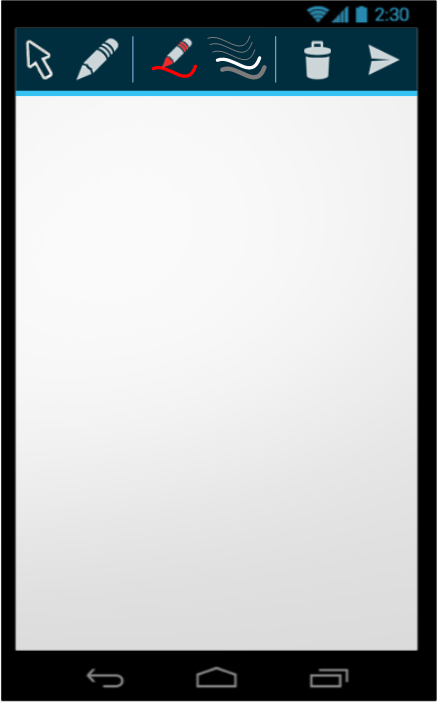
\includegraphics[width=\linewidth]{img/android/mockup_startscreen.png}
  \caption{Basic user interface (startscreen)}
  \label{fig:mockup_startscreen}
\end{figure}

\begin{figure}
  \centering
  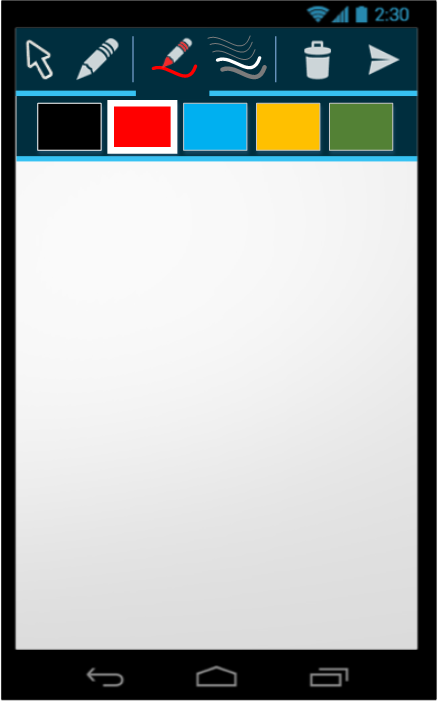
\includegraphics[width=\linewidth]{img/android/mockup_color.png}
  \caption{Select a color)}
  \label{fig:mockup_color}
\end{figure}

\begin{figure}
  \centering
  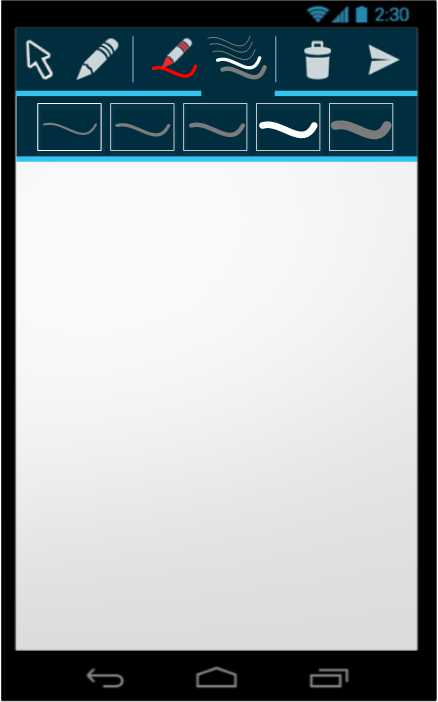
\includegraphics[width=\linewidth]{img/android/mockup_pen.png}
  \caption{Select a pen}
  \label{fig:mockup_pen}
\end{figure}

% =============================================================================
\section{Ergebnisse der Studie}
% =============================================================================
Blubb
% TODO: Bla bla bla

% =============================================================================
\section{Diskussion}
% =============================================================================
Bei der Studie hat sich unter anderem gezeigt, dass, entgegen unserer Erwartungen, die meisten Nutzer für das Auslösen der Übertragung zum Laptop keine Bewegungsgeste mit dem Smartphone sondern eher einen zu betätigenden Button bevorzugen. Dies ist auf den ersten Blick überraschend, zeigen mehrere Studien [TODO] doch ausführlich, dass Bewegungsgesten sehr natürlich sind. Jedoch sind Benutzer von Computern an die seit Jahren praktisch überall eingesetzte Maus- und Tastatur-Steuerung gewöhnt, bei der die Bedienung durch das Drücken von Buttons mit der Maus erfolgt. Diese hat sich auch auf Smartphones übertragen, nur werden die Buttons dort per Touchscreen direkt mit dem Finger bedient. Durch diese jahrelange Gewöhnung sehen geübte Benutzer diese Bedienung wohl als völlig natürlich an und empfinden dann daher auch das Betätigen eines Buttons als einfache und benutzerfreundliche Geste. Bewegungsgesten mit dem Smartphone wären damit eher eine Umstellung, auch wenn der Wow-Effekt natürlich größer wäre als beim Betätigen eines Buttons.
%% TODO: Anpassen an konkrete Ergebnisse der Studie und Erweitern


% =============================================================================
\section{Konklusion}
% =============================================================================
In diesem Paper haben wir unser Projekt Copy-To-Clipboard vorgestellt, das wir im Rahmen der HCI-Vorlesung im Sommersemester 2013 an der Universität Augsburg durchgeführt haben. Dabei haben wir die wirkliche Durchführung des Projekts, also die Implementierung außen vor gelassen, und uns auf die HCI-Aspekte des Projekts beschränkt um den iterativen, nutzerzentrierten HCI-Designprozess zu verstehen und anzuwenden.
% TODO: Bla bla bla



\balance
\bibliographystyle{acm-sigchi}
\bibliography{sample}

\end{document}